\chapter{Branch \& Bound}\label{branch_and_bound}

Come anticipato nel capitolo precedente possiamo usare due formulazioni (Cut Set o Subtour elimination) per risolvere il TSP. Il nostro problema però, sta nel avere un numero esponenziale di vincoli per garantire la connettività della soluzione. In questo capitolo descriviamo un modo per risolvere questo problema descritto nel libro \cite{bertsimas}. Forniamo inoltre una nostra variazione dell’algoritmo derivante dall’analisi dell’efficienza di quello descritto nel libro.

\section{Branch \& Bound totale}

In questa sezione, presenteremo un algoritmo di branching che permette di ridurre il numero dei vincoli nel problema del TSP. L'algoritmo di branching è una tecnica di risoluzione che suddivide il problema originale in sottoproblemi più piccoli, riducendo in molti casi il costo della risoluzione. Nella nostra ambientazione del problema usiamo un grafo completo orientato quindi presentiamo brevemente la formulazione completa.

Con 4.a e 4.b ci assicuriamo che per ogni nodo ci sia esattamente un arco entrante e un arco uscente.
I vincoli 4.c ci garantiscono la connettività della soluzione in quanto impongono almeno un possibile cammino da un nodo ad ogni altro nodo e il loro numero è \begin{math}O(2^{|N|})\end{math}.

\[ x_{i_j} =
  \begin{cases}
    1       & \quad \text{se} \text{l'arco \begin{math}(i, j) \in E\end{math} fa parte del percorso ottimo}\\
    0  & \quad \text{altrimenti}
  \end{cases}
\]

\[
\text{minimize} \quad \sum_{i = 1}^{|N|}\sum_{j = 1}^{|N|} c_{i_j} x_{i_j}
\]

\begin{minipage}[t]{0.9\textwidth}
\[
\sum_{i = 1}^{|N|} x_{i_j} = 1, \quad  i = 1, \dots, |N| 
\]
\end{minipage}%
\begin{minipage}[t]{0.1\textwidth}
\vspace{0,4cm}
(4.a)
\end{minipage}

\begin{minipage}[t]{0.9\textwidth}
\[
\sum_{j = 1}^{|N|} x_{i_j} = 1, \quad  j = 1, \dots, |N|
\]
\end{minipage}%
\begin{minipage}[t]{0.1\textwidth}
\vspace{0,4cm}
(4.b)
\end{minipage}

\begin{minipage}[t]{0.9\textwidth}
\[
\sum_{(i, j) \in \delta^{+}(S)}  x_{i_j} \geq 1, \quad \forall S \subset N, S \ne \varnothing, S \ne N
\]
\end{minipage}%
\begin{minipage}[t]{0.1\textwidth}
\vspace{0,2cm}
(4.c)
\end{minipage}

\[
dove \quad \delta^{+}(S) = \{ (i,j) \in E: i \in S, j \notin S \}
\]

\begin{minipage}[t]{0.9\textwidth}
\[
x_a \in \{0, 1\}, \quad \forall a \in E
\]
\end{minipage}%
\begin{minipage}[t]{0.1\textwidth}
\vspace{0,1cm}
(4.d)
\end{minipage}

\subsection{Problema di assegnamento}
In \ref{elon_teletrasporto} (\nameref{elon_teletrasporto}) abbiamo già visto a cosa ci porta la rimozione dei vincoli di connessione. In particolare ci può portare ad una soluzione disconnessa e il problema restante prende il nome di Problema di Assegnamento (PA). La sua matrice dei vincoli è unimodulare e, quindi, la soluzione del rilassamento continuo è intera.

Possiamo procedere dicendo che la soluzione del PA sarà sicuramente un limite inferiore a quella del problema originale in quanto lo spazio ammissibile del TSP è compreso in quello del PA. Se la soluzione del PA produce un solo ciclo, allora sarà la soluzione ottima per il TSP. Altrimenti si avrà un insieme di cicli disgiunti in cui ogni nodo è visitato esattamente una volta.

Possiamo quindi pensare di risolvere il TSP usando il Branch and Bound, in cui i limiti inferiori sono calcolati risolvendo dei problemi di assegnamento. 

Nel branching si fissano a zero le variabili che possono rendere inammissibile la soluzione per il TSP, quindi quelle con valore 1 della soluzione al PA.

Nella figura \ref{img:es_sol_disconnessa} notiamo che abbiamo due cicli nella soluzione per il PA. Il numero di nodi è 8, quindi creiamo 8 nodi figli e per ogni problema cerchiamo di aprire uno dei archi del percorso proposto dalla soluzione del PA.

Fortunatamente non si avrà la necessità di visitare, e quindi anche costruire, tutto l'albero, in quanto possiamo potare alcune sue parti a priori. In particolare un nodo non genera figli se:

\begin{itemize}
    \item se la soluzione per il PA è ammissibile per il TSP
    \item se la soluzione del PA è inammissibile
    \item se la soluzione del PA è inammissibile per il TSP ed è peggiore della migliore soluzione ammissibile per il TSP finora trovata
\end{itemize}

\newpage
Forniamo il pseudocodice dell'algoritmo che abbiamo sviluppato.

\begin{algorithm}
\caption{Branch and Bound for TSP}\label{alg:brand:and_bound_pseudocode}
\begin{algorithmic}
\State $best\_solution \gets None$
\State $best\_objective\_value \gets +\infty$
\State $stack \gets$ a list with only one model for PA
\While{$stack$ is not empty}
    \State $current\_model \gets stack.pop()$
    \State $solution \gets current.solve()$
    \If{$solution$ is None}
        continue  \Comment{Infeasible solution, backtrack}
    \EndIf
    \State $objective\_value \gets solution.get\_objective\_value()$
    \If{$objective\_value \geq best\_objective\_value$}
        continue  \Comment{Solution is worse than the best found so far, backtrack}
    \EndIf
    \If{the number of cicles is 1}\Comment{Found a feasible solution with lower objective value}
        \State $best\_solution \gets solution$
        \State $best\_objective\_value \gets objective\_value$
    \EndIf
    \For{$(i, j) \in (1\dots N) \times (1\dots N)$}
        \If{$i \ne j$ and $x_{i_j}$ is an arc in the current solution}
            \State Create a new model cloning the previous one
            \State Add constrain $x_{i_j} = 0$ to the new model
            \State Push the new model to the stack
        \EndIf
    \EndFor
\EndWhile
\If{$best\_solution$ is None}
        \State raise error "Infeasible"
\EndIf \\
\Return$best\_solution$
\end{algorithmic}
\end{algorithm}

\section{Branch \& Bound con branching parziale}
Dopo aver implementato l’algoritmo descritto nella sezione precedente abbiamo eseguito dei test. Pur ottenendo dei buoni risultati per alcuni casi di studio abbiamo notato un degrado considerevole delle prestazioni in altri. Dopo aver investigato sulla natura del problema abbiamo concluso che la principale causa era la forte frammentazione dell’albero indotta dal generare un numero |N| di figli per ogni iterazione nella quale veniva eseguito il branching. 

Proponiamo quindi un modo alternativo, che sfrutta le stesse idee descritte prima, ma che esegue il branching solo su due variabili decisionali che nella soluzione corrente, non ammissibile del problema viaggiatore, rappresentano due degli archi scelti.

Forniamo inoltre, un'analisi delle prestazioni dei due algoritmi su diverse istanze del problema. Abbiamo scelto di utilizzare 15 nodi e nella tabella \ref{tab:bb_performance} rappresentiamo il tempo impiegato e il numero dei nodi esplorati. Il numero dei nodi aggiunti può essere visto anche come numero dei vincoli usati per garantire la connessione.

\begin{table}[htbp]
    \centering
    \begin{tabular}{|c|c|c|c|c|}
        \hline
        \textbf{ID} & \textbf{B\&B Time (s)} & 
        \textbf{\# added nodes} & 
        \textbf{Binary B\&B Time (s)} & 
        \textbf{\# added nodes} \\
        \hline
        1 & 13.14 & 300  & 0.28 & 6 \\
        \hline
        2 & 3.26 & 75 & 0.19 & 4 \\
        \hline
        3 & 2.064 & 45 & 0.65 & 14\\
        \hline
        4 & 2.78 & 60 & 0.11 & 2\\
        \hline
        5 & 686.72 & 11370 & 5.64 & 118 \\
        \hline
        6 & 1.73 & 30 & 0.32 & 4 \\
        \hline
        7 & 37.71 & 420 & 2.47 & 42 \\
        \hline
        8 & 12.06 & 240 & 1.52 & 22 \\
        \hline
        9 & 35.92 & 585 & 2.09 & 38 \\
        \hline
        10 & 8.58 & 195 & 6.31 & 146 \\
        \hline
    \end{tabular}
    \caption{I due Branch and Bound a confronto}\label{tab:bb_performance}
\end{table}


\section{Applicazione al caso di studio di Elon Musk}
Nella sezione precedente, abbiamo presentato come possiamo gestire il numero esponenziale di vincoli per garantire una soluzione connessa nel TSP tramite un algoritmo di branching. In questa sezione esaminiamo passo passo l’esecuzione dell'algoritmo di branching binario sulla nostra ambientazione del problema.

\subsection{Definizione del problema}

Consideriamo un grafo completo in cui i nodi rappresentano i pianeti del nostro sistema solare e gli archi rappresentano i percorsi tra i pianeti. Ogni arco ha associato un costo. L'obiettivo è determinare il percorso chiuso di costo minimo che permetta a Elon Musk di visitare tutti i pianeti una sola volta, tornando infine al pianeta di partenza.

Il grafo, nel nostro caso è un grafo orientato in quanto il costo può differire scambiando il pianeta di partenza e quello di arrivo. In particolare il costo del viaggio dipende dai seguenti fattori:

\begin{itemize}
    \item distanza
    \item numero degli asteroidi sul percorso
    \item orientazione della navicella rispetto alla direzione della luce (la navicella di Elon vuole sprecare meno energia elettrica possibile acquisendone il più possibile dai raggi solari)
\end{itemize}

\[
costo = w1 * dist\_norm + w2 * num\_ast\_norm + w3 * angolo\_trasformato 
\]

\[
dist\_norm = (distanza - distanza\_min) / (distanza\_max - distanza\_min)
\]

\[
num\_ast\_norm = (num\_ast - num\_ast_min) / (num\_ast\_max - num\_ast\_min)
\]

\[
angolo\_trasformato = angolo / 180^{\circ}
\]

dove w1, w2 e w3 rappresentano i pesi che diamo a ciascun parametro che influenza il costo finale.


\subsection{Esecuzione dell'algoritmo}
Andiamo a vedere le decisioni che prende l'algoritmo su ciascun nodo dell'albero. Rappresentiamo l'albero in Figura \ref{img:albero}), nel quale i nodi sono numerati nello stesso ordine nel quale vengono visitati.

\begin{itemize}
    \item Al nodo 1 come si può vedere nell'immagine \ref{img:es_space_sol_disconnessa} si ha una soluzione ammissibile per il PA, ma non per il TSP. 117 quindi è un limite inferiore alla soluzione del problema originario e si hanno due nuovi nodi: 2 e 3. Nelle fasi successive andiamo a migliorare sempre di più i limiti inferiori per poi raggiungere la soluzione ottima.
    \item Lo stesso avviene per i nodi 2 e 3. Hanno una soluzione ammissibile per il problema di PA, ma non per il TSP, quindi generano entrambi due figli.
    \item Il nodo 4 individua una soluzione ammissibile (rappresentata in figura \ref{img:es_space_sol_connessa}) per il problema di TSP, per ora è la soluzione migliore, quindi viene aggiornata. Siccome si ha una soluzione ammissibile per il problema di TSP, il nodo 4 non genera figli.
    \item Negli altri nodi (5, 6, 7) la soluzione è peggiore di quella che è stata già trovata al nodo 4, quindi non generano figli.
\end{itemize}

\begin{figure}[ht]
	\centering
	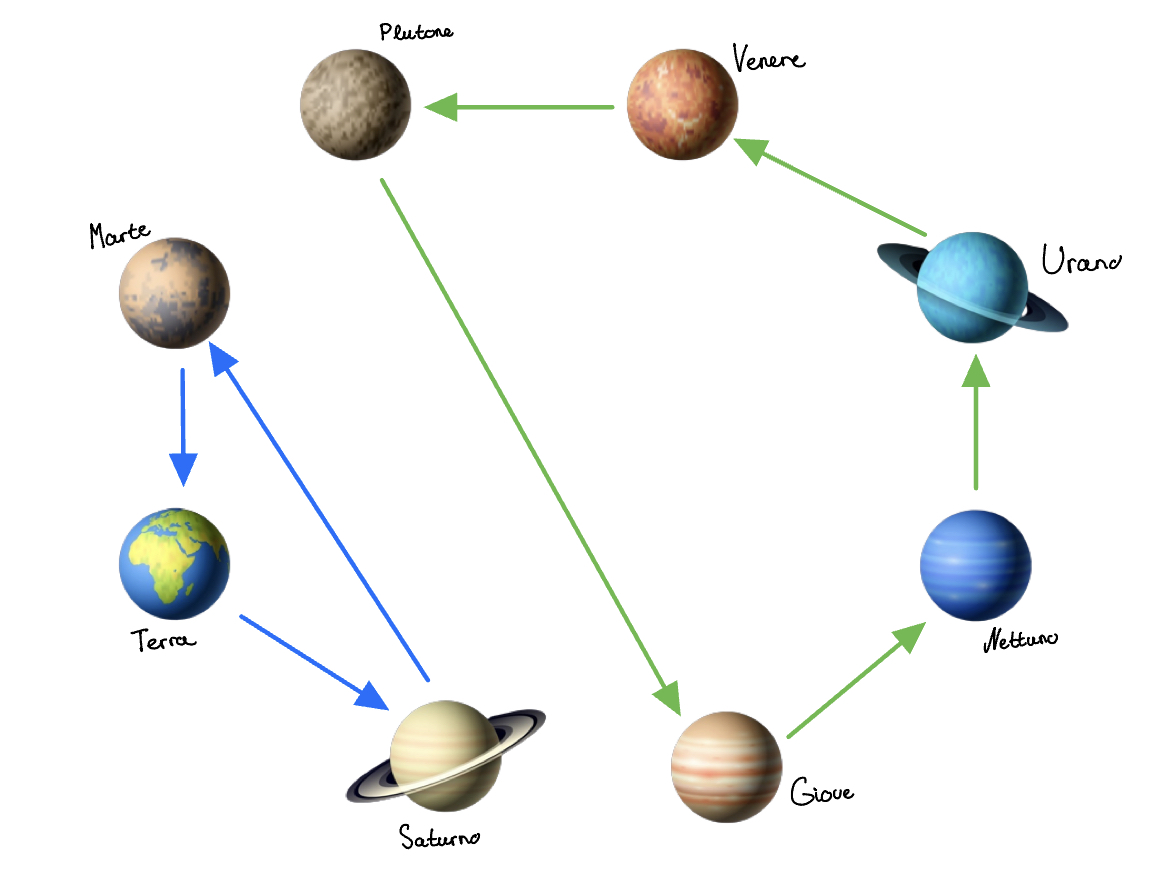
\includegraphics[width=1\columnwidth]{images/es_space_sol_disconnessa}
	\caption{\textit{Soluzione al problema di Assegnamento al Nodo 1}}
	\label{img:es_space_sol_disconnessa}
\end{figure}

\begin{figure}[ht]
	\centering
	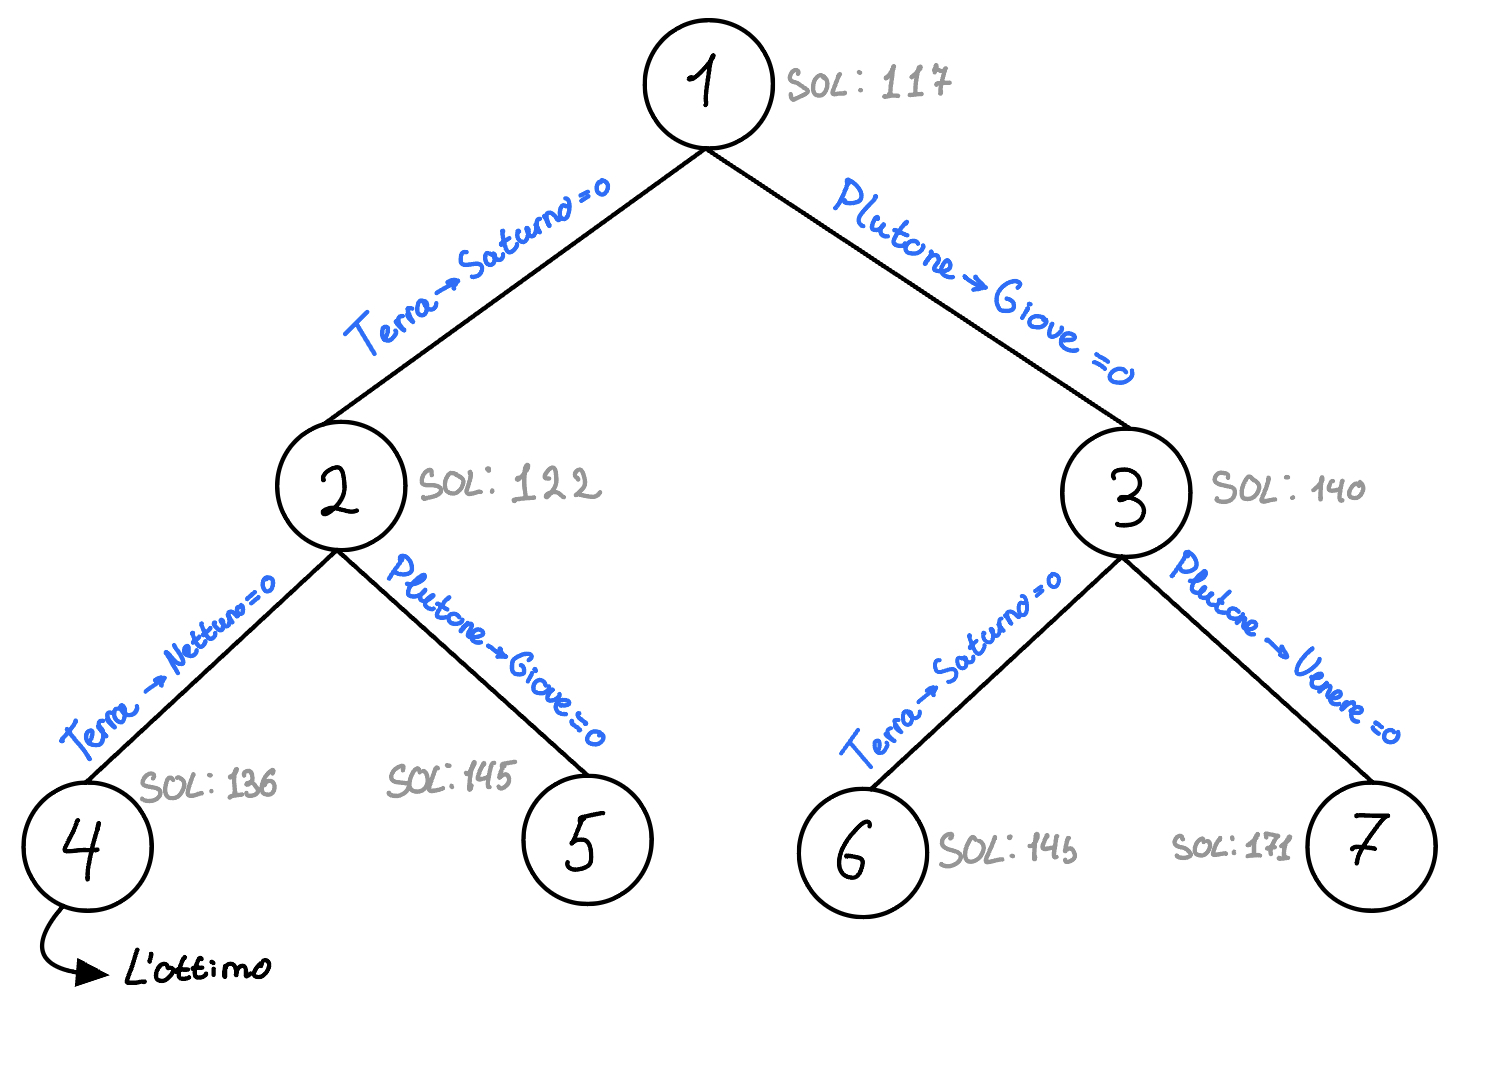
\includegraphics[width=1\columnwidth]{images/albero}
	\caption{\textit{Albero creato dall'algoritmo di branching}}
	\label{img:albero}
\end{figure}

\begin{figure}[ht]
	\centering
	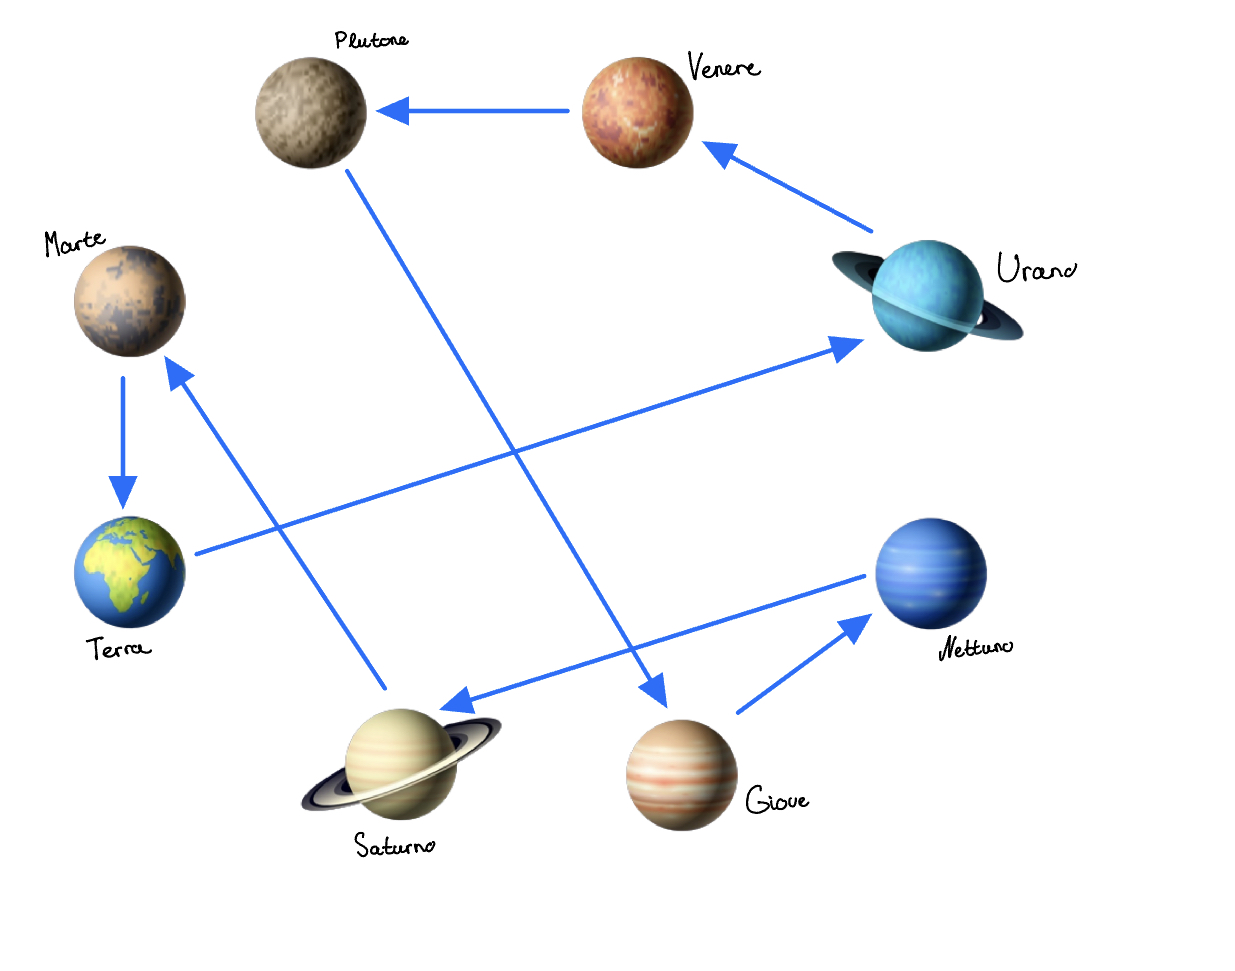
\includegraphics[width=1\columnwidth]{images/es_space_sol_connessa}
	\caption{\textit{Soluzione finale al problema del TSP}}
	\label{img:es_space_sol_connessa}
\end{figure}